% Gabarit pandoc des corrigés publiés (brut et guidé). Contenu sans marque ni nom de site.
% Compilation : lualatex (latexmk -lualatex).
% Le Markdown reste la source unique : ne pas éditer ce fichier .tex à la main.
\documentclass[11pt,a4paper]{article}

% --- Moteur, polices (Latin Modern) et langue ---------------------------------
\usepackage{iftex}
\ifLuaTeX\else\errmessage{Ce document se compile avec lualatex}\fi
\usepackage{amsmath,amssymb,mathtools}
\usepackage{fontspec}
% mathrm=sym : \mathrm prend ses glyphes dans la police mathématique (ℓ, μ, Ω), comme KaTeX.
\usepackage[math-style=TeX,bold-style=TeX,mathrm=sym]{unicode-math}
% Repli pour les glyphes absents de Latin Modern (indices et exposants Unicode,
% flèches, filets des schémas en texte, symboles) : DejaVu, puis Latin Modern Math
% (ℓ, lettres mathématiques Unicode des légendes).
\directlua{
  luaotfload.add_fallback("repliTexte", {"DejaVuSerif:mode=harf;", "DejaVuSans:mode=harf;", "file:latinmodern-math.otf:mode=harf;"})
  luaotfload.add_fallback("repliMono", {"DejaVuSansMono:mode=harf;", "DejaVuSans:mode=harf;", "file:latinmodern-math.otf:mode=harf;"})
}
\setmainfont{Latin Modern Roman}[RawFeature={fallback=repliTexte}]
\setsansfont{Latin Modern Sans}[RawFeature={fallback=repliTexte}]
\setmonofont{Latin Modern Mono}[RawFeature={fallback=repliMono}]
\setmathfont{Latin Modern Math}
\usepackage[french]{babel}
\frenchsetup{SmallCapsFigTabCaptions=false}

% --- Mise en page --------------------------------------------------------------
\usepackage[a4paper,margin=2.2cm,headheight=14pt,footskip=1.2cm]{geometry}
\usepackage{microtype}
\setlength{\emergencystretch}{4em}
\tolerance=1500
\setlength{\parindent}{0pt}
\setlength{\parskip}{0.55\baselineskip plus 2pt minus 1pt}
\usepackage{xcolor}
% Gris nommés : babel-french rend « ! » actif dans le document.
\definecolor{gris2}{gray}{0.98}
\definecolor{gris3}{gray}{0.97}
\definecolor{gris5}{gray}{0.95}
\definecolor{gris35}{gray}{0.65}
\definecolor{gris40}{gray}{0.60}
\definecolor{gris45}{gray}{0.55}
\definecolor{gris50}{gray}{0.50}
\definecolor{gris55}{gray}{0.45}
\definecolor{gris60}{gray}{0.40}
\definecolor{gris65}{gray}{0.35}
\definecolor{gris70}{gray}{0.30}
\definecolor{gris80}{gray}{0.20}
\definecolor{gris85}{gray}{0.15}
\usepackage{graphicx}
\usepackage{float}
\usepackage{caption}
\captionsetup{font=small,labelformat=empty,justification=centering}
\usepackage{booktabs,longtable,array,multirow,calc}
\usepackage{siunitx}
\sisetup{locale=FR}
\usepackage[version=4]{mhchem}
\usepackage{listings}
\usepackage{fancyhdr}
\usepackage{lastpage}
\usepackage[most]{tcolorbox}
\usepackage{enumitem}
\setlist{nosep,leftmargin=*,topsep=2pt}
\usepackage[hidelinks,unicode]{hyperref}
\usepackage{bookmark}
\hypersetup{pdftitle={Mines-Ponts PC — Maths 1 2026},pdfauthor={Rédigé par IA},pdfcreator={LaTeX},pdfsubject={Corrigé brut}}
\usepackage{xurl}

% --- Pandoc : listes, tableaux, figures ----------------------------------------
\providecommand{\passthrough}[1]{#1}
\providecommand{\tightlist}{\setlength{\itemsep}{0pt}\setlength{\parskip}{0pt}}

\makeatletter
\def\maxwidth{\ifdim\Gin@nat@width>\linewidth\linewidth\else\Gin@nat@width\fi}
\def\maxheight{\ifdim\Gin@nat@height>0.55\textheight 0.55\textheight\else\Gin@nat@height\fi}
\makeatother
\setkeys{Gin}{width=\maxwidth,height=\maxheight,keepaspectratio}
\setcounter{secnumdepth}{-\maxdimen}
\providecommand{\pandocbounded}[1]{#1}

% --- Code (listings) -----------------------------------------------------------
\lstset{
  basicstyle=\ttfamily\small,
  columns=fullflexible,
  keepspaces=true,
  breaklines=true,
  breakatwhitespace=false,
  postbreak=\mbox{\textcolor{gris50}{$\hookrightarrow$}\space},
  frame=single,
  rulecolor=\color{gris35},
  framesep=4pt,
  xleftmargin=5pt,xrightmargin=5pt,
  backgroundcolor=\color{gris3},
  keywordstyle=\bfseries,
  commentstyle=\color{gris65},
  stringstyle=\color{gris80},
  showstringspaces=false,
  tabsize=4,
  extendedchars=true,
  aboveskip=6pt,belowskip=6pt,
}

% --- Macros des corrigés (KaTeX ↔ LaTeX) ---------------------------------------
% Les corrigés sont écrits pour KaTeX : on définit ici ce que KaTeX connaît et
% que LaTeX n'a pas, sans jamais retoucher le Markdown.
\providecommand{\R}{\mathbb{R}}
\providecommand{\N}{\mathbb{N}}
\providecommand{\Z}{\mathbb{Z}}
\providecommand{\Q}{\mathbb{Q}}
\providecommand{\C}{\mathbb{C}}
\providecommand{\dd}{\mathrm{d}}
\providecommand{\llbracket}{\lBrack}
\providecommand{\rrbracket}{\rBrack}
\providecommand{\lBrace}{\lbrace}
\providecommand{\rBrace}{\rbrace}
\providecommand{\Box}{\square}
\providecommand{\Diamond}{\lozenge}
\providecommand{\varnothing}{\emptyset}
\providecommand{\argmax}{\operatorname*{arg\,max}}
\providecommand{\argmin}{\operatorname*{arg\,min}}
\renewcommand{\leq}{\leqslant}
\renewcommand{\geq}{\geqslant}

% Équation hors texte : réduite à la largeur de la ligne si elle déborde.
\newsavebox{\boiteequation}
\newcommand{\equationajustee}[1]{%
  \sbox{\boiteequation}{$\displaystyle #1$}%
  \ifdim\wd\boiteequation>\linewidth
    \[\resizebox{\linewidth}{!}{\usebox{\boiteequation}}\]%
  \else
    \[#1\]%
  \fi}

% --- Encadrés pédagogiques (sobres, lisibles en noir et blanc) -----------------
\tcbset{
  encadre/.style={
    enhanced,breakable,sharp corners,
    colback=white,colframe=gris55,
    boxrule=0.4pt,leftrule=2.2pt,
    left=6pt,right=6pt,top=3pt,bottom=3pt,
    before skip=6pt,after skip=6pt,
    fonttitle=\bfseries\small,coltitle=black,
    attach title to upper,after title={\quad},
    parbox=false,
  }
}
\newtcolorbox{indication}[1]{encadre,colframe=gris45,colback=gris2,title={Indication~#1}}
\newtcolorbox{methode}{encadre,colframe=gris70,title={Méthode}}
\newtcolorbox{piege}{encadre,colframe=gris85,boxrule=0.8pt,leftrule=2.2pt,title={Piège}}
\newtcolorbox{jury}{encadre,colframe=gris60,colback=gris5,title={Jury}}
\newtcolorbox{encadrenote}{encadre,colframe=gris40}

% --- Titres de section ---------------------------------------------------------
\usepackage{titlesec}
\titleformat{\section}{\Large\bfseries}{}{0pt}{}
\titleformat{\subsection}{\large\bfseries}{}{0pt}{}
\titleformat{\subsubsection}{\normalsize\bfseries}{}{0pt}{}
\titlespacing*{\section}{0pt}{14pt plus 4pt minus 2pt}{6pt}
\titlespacing*{\subsection}{0pt}{10pt plus 3pt minus 2pt}{4pt}
\titlespacing*{\subsubsection}{0pt}{8pt plus 2pt minus 2pt}{2pt}

% --- En-tête et pied de page ---------------------------------------------------
\pagestyle{fancy}
\fancyhf{}
\fancyhead[L]{\small\textsc{Corrigé brut} · Mines-Ponts PC}
\fancyhead[R]{\small Maths 1 2026}
\fancyfoot[L]{\footnotesize Corrigé rédigé par IA, non officiel}
\fancyfoot[R]{\footnotesize \thepage\,/\,\pageref*{LastPage}}
\renewcommand{\headrulewidth}{0.4pt}
\renewcommand{\footrulewidth}{0pt}
\fancypagestyle{plain}{\fancyhf{}\fancyfoot[R]{\footnotesize \thepage\,/\,\pageref*{LastPage}}\fancyfoot[L]{\footnotesize Corrigé rédigé par IA, non officiel}\renewcommand{\headrulewidth}{0pt}}

\begin{document}
\thispagestyle{plain}
\begin{center}
  {\small\scshape Corrigé brut}\par\smallskip
  {\LARGE\bfseries Mines-Ponts PC — Maths 1 2026\par}\medskip
  {\large Mines-Ponts · PC · Maths 1 · 2026\par}
\end{center}
\vspace{2pt}\hrule\vspace{8pt}

\emph{Corrigé rédigé par IA, non officiel. Signalez toute erreur.}

\textbf{Sommes d'endomorphismes de carré nul.} Durée 3 h, calculatrice interdite. Tous les espaces sont des \(\mathbb C\)-espaces vectoriels de dimension finie.

On note \(\mathcal C(E)=\{u\in\mathcal L(E):u^2=0\}\) et \(\Sigma_p\mathcal C(E)\) l'ensemble des sommes de \(p\) éléments de \(\mathcal C(E)\). Enfin \(\Sigma_\infty\mathcal C(E)=\bigcup_{p\ge1}\Sigma_p\mathcal C(E)\).

\hypertarget{a-ruxe9duction-des-endomorphismes-de-carruxe9-nul}{%
\section{A --- Réduction des endomorphismes de carré nul}\label{a-ruxe9duction-des-endomorphismes-de-carruxe9-nul}}

\(E\) est de dimension \(n>0\), \(u\in\mathcal L(E)\) vérifie \(u^2=0\) et \(u\neq0\) ; on note \(r=\operatorname{rg}(u)\).

\hypertarget{question-1}{%
\subsection{Question 1}\label{question-1}}

Soit \(\lambda\) une valeur propre de \(u\) et \(x\neq0\) tel que \(u(x)=\lambda x\). Alors \(0=u^2(x)=\lambda^2x\).

Comme \(x\neq0\), on obtient \(\lambda=0\).

La seule valeur propre possible est donc \(0\), et c'en est bien une : \(\chi_u\) est de degré \(n\ge1\), donc admet une racine dans \(\mathbb C\).

Ainsi \(\operatorname{Sp}(u)=\{0\}\) et, \(\chi_u\) étant scindé, \(\chi_u=X^n\).

Sur \(\mathbb C\), \(\chi_u\) est scindé, \(u\) est trigonalisable, et la trace est la somme des valeurs propres comptées avec leur multiplicité. D'où
\equationajustee{\boxed{\begin{aligned}{}&\operatorname{Sp}(u)=\{0\},\\ &\operatorname{tr}(u)=0.\end{aligned}}}

\hypertarget{question-2}{%
\subsection{Question 2}\label{question-2}}

Si \(y=u(x)\in\operatorname{Im}u\), alors \(u(y)=u^2(x)=0\) : \(\operatorname{Im}u\subset\operatorname{Ker}u\).

Par le théorème du rang, \(\dim\operatorname{Ker}u=n-r\), donc \(r\le n-r\), soit
\equationajustee{\boxed{r\le\frac n2.}}

\hypertarget{question-3}{%
\subsection{Question 3}\label{question-3}}

En dimension finie, \(\operatorname{Ker}u\) admet un supplémentaire \(S\), de dimension \(n-(n-r)=r\), avec \(r\ge1\) puisque \(u\neq0\).

Une base \((e_1,\dots,e_r)\) de \(S\) est une famille libre telle que \(\operatorname{Ker}(u)\oplus\operatorname{Vect}(e_1,\allowbreak \dots,\allowbreak e_r)=E\).

Soient \(\lambda_1,\dots,\lambda_r\) tels que \(\sum_i\lambda_iu(e_i)=0\). Le vecteur \(x=\sum_i\lambda_ie_i\) vérifie \(u(x)=0\).

Ainsi \(x\in\operatorname{Ker}u\cap S=\{0\}\), donc \(x=0\), et la liberté de \((e_i)\) donne \(\lambda_i=0\) pour tout \(i\). \textbf{La famille \((u(e_1),\dots,u(e_r))\) est libre.}

\hypertarget{question-4}{%
\subsection{Question 4}\label{question-4}}

La famille \((u(e_1),\dots,u(e_r))\) est libre et contenue dans \(\operatorname{Im}u\), de dimension \(r\) : c'est une base de \(\operatorname{Im}u\).

Comme \(\operatorname{Im}u\subset\operatorname{Ker}u\) (Q2), on la complète en une base \((u(e_1),\dots,u(e_r),f_1,\dots,f_{n-2r})\) \textbf{de \(\operatorname{Ker}u\)} (aucun \(f_j\) si \(n=2r\)).

Comme \(E=S\oplus\operatorname{Ker}u\), la concaténation
\equationajustee{\mathcal B=(e_1,\dots,e_r,\;u(e_1),\dots,u(e_r),\;f_1,\dots,f_{n-2r})}
est une base de \(E\).

Lisons les colonnes. Pour \(i\le r\), \(u(e_i)\) est le \((r+i)\)-ième vecteur de \(\mathcal B\).

Ensuite \(u(u(e_i))=u^2(e_i)=0\). Enfin \(u(f_j)=0\) car \(f_j\in\operatorname{Ker}u\). D'où
\equationajustee{\boxed{\operatorname{Mat}_{\mathcal B}(u)=\begin{pmatrix}0_r&0_r&(0)\\ I_r&0_r&(0)\\ (0)&(0)&0_{n-2r}\end{pmatrix}.}}

\begin{figure}[H]
\centering
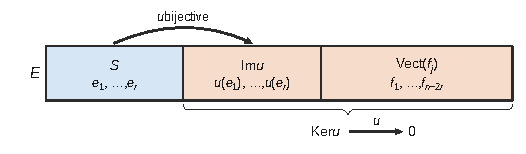
\includegraphics{figures/q4-structure-carre-nul.pdf}
\caption*{Figure 1 --- Base adaptée de Q4 : u envoie bijectivement S sur Im u et
annule Ker u = Im u ⊕ Vect(f\_j), les cases suivant l'ordre de la base}
\end{figure}

\hypertarget{question-5}{%
\subsection{Question 5}\label{question-5}}

Notons \(M_m\) la matrice par blocs de l'énoncé (\(1\le m\le n/2\)).

\emph{Existence} : \(m=r\) convient (Q4), et \(r>0\) car \(u\neq0\).

\emph{Unicité} : les \(m\) premières colonnes de \(M_m\) sont les vecteurs \(\varepsilon_{m+1},\dots,\varepsilon_{2m}\) de la base canonique, les autres sont nulles. Donc \(\operatorname{rg}M_m=m\).

Si \(u\) est représenté par \(M_m\) dans une base, alors \(m=\operatorname{rg}M_m=\operatorname{rg}u=r\), car le rang d'un endomorphisme est celui de sa matrice dans toute base. Donc
\equationajustee{\boxed{m=r=\operatorname{rg}(u)\ \text{est l'unique entier convenable.}}}

\hypertarget{b-somme-dun-nombre-arbitraire-dendomorphismes-de-carruxe9-nul}{%
\section{B --- Somme d'un nombre arbitraire d'endomorphismes de carré nul}\label{b-somme-dun-nombre-arbitraire-dendomorphismes-de-carruxe9-nul}}

\(E\) est de dimension \(n\ge2\) et \(\mathcal H(E)=\{u\in\mathcal L(E):\operatorname{tr}u=0\}\). On utilise la règle \(E_{i,j}E_{k,l}=\delta_{j,k}E_{i,l}\).

\hypertarget{question-6}{%
\subsection{Question 6}\label{question-6}}

Par la règle rappelée, \((E_{i,j})^2=\delta_{j,i}E_{i,j}\). C'est \(E_{i,i}\neq0\) si \(i=j\), et \(0\) si \(i\neq j\).
\equationajustee{\boxed{(E_{i,j})^2=0\iff i\neq j.}}

Soient \(i\neq j\). La matrice \(F_{i,j}\) est nulle hors des lignes et colonnes \(i\) et \(j\).

L'endomorphisme \(f\) de \(\mathbb C^n\) associé annule les \(\varepsilon_k\) pour \(k\notin\{i,j\}\), et
\equationajustee{\begin{aligned}f(\varepsilon_i)&=\varepsilon_i-\varepsilon_j,\\ f(\varepsilon_j)&=\varepsilon_i-\varepsilon_j.\end{aligned}}

Alors \(f^2(\varepsilon_i)=f^2(\varepsilon_j)=f(\varepsilon_i)-f(\varepsilon_j)=0\), et \(f^2(\varepsilon_k)=0\) pour les autres \(k\).

Autrement dit, dans \((\varepsilon_i,\varepsilon_j)\), le bloc utile est \(\begin{pmatrix}1&1\\-1&-1\end{pmatrix}\), de carré nul. Les produits ne commutant pas, on ne développe pas \(F_{i,j}^2\) par une identité remarquable.
\equationajustee{\boxed{\forall i\neq j,\quad (F_{i,j})^2=0_n.}}

\hypertarget{question-7}{%
\subsection{Question 7}\label{question-7}}

Soit \(A=(a_{i,j})\in\mathcal H_n\), donc \(a_{n,n}=-\sum_{i=1}^{n-1}a_{i,i}\).

Pour \(i\le n-1\), la définition de \(F_{i,n}\) donne
\equationajustee{E_{i,i}-E_{n,n}=F_{i,n}-E_{i,n}+E_{n,i}.}

La partie diagonale de \(A\) s'écrit donc
\equationajustee{\begin{aligned}\sum_{i=1}^na_{i,i}E_{i,i}&=\sum_{i=1}^{n-1}a_{i,i}(E_{i,i}-E_{n,n})\\ &=\sum_{i=1}^{n-1}a_{i,i}\big(F_{i,n}-E_{i,n}+E_{n,i}\big),\end{aligned}}
et
\equationajustee{\boxed{\begin{aligned}A={}&\sum_{i\neq j}a_{i,j}E_{i,j}+\sum_{i=1}^{n-1}a_{i,i}F_{i,n}\\ &-\sum_{i=1}^{n-1}a_{i,i}E_{i,n}+\sum_{i=1}^{n-1}a_{i,i}E_{n,i},\end{aligned}}}
combinaison linéaire de matrices \(E_{i,j}\) (\(i\neq j\)) et \(F_{i,n}\) (\(1\le i\le n-1\)).

\hypertarget{question-8}{%
\subsection{Question 8}\label{question-8}}

On procède par double inclusion.

\emph{\(\Sigma_\infty\mathcal C(E)\subset\mathcal H(E)\).} Soit \(u=u_1+\dots+u_p\) avec \(u_k^2=0\).

Chaque \(u_k\) est de trace nulle (Q1 si \(u_k\neq0\), évident si \(u_k=0\)), donc \(\operatorname{tr}u=0\) par linéarité de la trace.

\emph{\(\mathcal H(E)\subset\Sigma_\infty\mathcal C(E)\).} Soit \(u\in\mathcal H(E)\) et \(A\) sa matrice dans une base \(\mathcal B\) fixée : \(\operatorname{tr}A=0\).

Par Q7, \(A=\sum_k\lambda_kM_k\) où chaque \(M_k\) est un \(E_{i,j}\) (\(i\neq j\)) ou un \(F_{i,n}\), donc de carré nul (Q6).

Comme \((\lambda_kM_k)^2=\lambda_k^2M_k^2=0\), la matrice \(A\) est une somme finie de matrices de carré nul.

L'application \(f\mapsto\operatorname{Mat}_{\mathcal B}(f)\) étant un isomorphisme d'algèbres, \(u\) est une somme finie d'éléments de \(\mathcal C(E)\). Les deux inclusions donnent
\equationajustee{\boxed{\Sigma_\infty\mathcal C(E)=\mathcal H(E).}}

\hypertarget{c-somme-de-trois-endomorphismes-de-carruxe9-nul}{%
\section{C --- Somme de trois endomorphismes de carré nul}\label{c-somme-de-trois-endomorphismes-de-carruxe9-nul}}

\(E\) est de dimension \(n\ge5\) ; \(u\) est de trace nulle, \(1\) est valeur propre de \(u\) et \(d=\dim\operatorname{Ker}(u-{\mathrm{id}}_E)>\frac{3n}4\).

\hypertarget{question-9}{%
\subsection{Question 9}\label{question-9}}

\emph{Rôle de \(n\ge5\).} Pour tout \(u\) de trace nulle, \(u\neq{\mathrm{id}}_E\) car \(\operatorname{tr}({\mathrm{id}}_E)=n\neq0\). Donc \(d\le n-1\).

Les contraintes imposent alors \(n-1\ge d>\frac{3n}4\), soit \(n>4\) : elles ne peuvent être satisfaites que si \(n\ge5\).

\emph{Construction.} Dans une base \((\varepsilon_1,\dots,\varepsilon_n)\), soit \(u\) de matrice \(D=\operatorname{diag}(1,\dots,1,-(n-1))\), avec \(n-1\) fois la valeur \(1\).

Alors \(\operatorname{tr}u=(n-1)-(n-1)=0\).

Comme \(-(n-1)\neq1\), la matrice \(D-I_n=\operatorname{diag}(0,\dots,0,-n)\) est de rang \(1\). Donc \(d=n-1\), et \(1\) est valeur propre.

Enfin
\equationajustee{n-1>\frac{3n}4\iff n>4,}
vrai car \(n\ge5\). \textbf{Un tel endomorphisme existe.}

\hypertarget{question-10}{%
\subsection{Question 10}\label{question-10}}

On pose \(w=u-{\mathrm{id}}_E\). Comme \(\operatorname{Ker}w=\operatorname{Ker}(u-{\mathrm{id}}_E)\) est de dimension \(d\), le théorème du rang donne \(\operatorname{rg}w=n-d<\frac n4\).

Comme \(v^2=0\), et sans supposer que \(v\) et \(w\) commutent :
\equationajustee{\begin{aligned}(w-v)^2&=w^2-wv-vw+v^2\\ &=w\circ(w-v)-v\circ w.\end{aligned}}

\emph{Sous-additivité du rang.} Pour \(f,g\in\mathcal L(E)\), on a \(\operatorname{Im}(f+g)\subset\operatorname{Im}f+\operatorname{Im}g\).

La réunion d'une base de \(\operatorname{Im}f\) et d'une base de \(\operatorname{Im}g\) engendre \(\operatorname{Im}f+\operatorname{Im}g\). Donc
\equationajustee{\operatorname{rg}(f+g)\le\dim(\operatorname{Im}f+\operatorname{Im}g)\le\operatorname{rg}f+\operatorname{rg}g.}

\emph{Rang d'une composée} (cours de première année) : \(\operatorname{rg}(f\circ g)\le\min(\operatorname{rg}f,\allowbreak \operatorname{rg}g)\).

D'où \(\operatorname{rg}\big(w\circ(w-v)\big)\le\operatorname{rg}w\) et \(\operatorname{rg}(v\circ w)\le\operatorname{rg}w\), puis
\equationajustee{\operatorname{rg}\big((w-v)^2\big)\le2\operatorname{rg}w<\frac n2.}
\equationajustee{\boxed{\operatorname{rg}\big((w-v)^2\big)<\frac n2.}}

\hypertarget{question-11}{%
\subsection{Question 11}\label{question-11}}

Soit \(K=\operatorname{Ker}\big((w-v)^2\big)\), de dimension \(k=n-\operatorname{rg}\big((w-v)^2\big)\). Par Q10, \(k>\frac n2>0\).

\emph{Stabilité.} Si \(x\in K\), alors
\equationajustee{(w-v)^2\big((w-v)(x)\big)=(w-v)\big((w-v)^2(x)\big)=0,}
donc \((w-v)(x)\in K\) : \(K\) est stable par \(w-v\).

L'endomorphisme \(g\) induit par \(w-v\) sur \(K\) vérifie \(g^2=0\). Par Q1 si \(g\ne0\) (évident sinon), \(\chi_g=X^k\).

Comme \(u-v=(w-v)+{\mathrm{id}}_E\), \(K\) est stable par \(u-v\), qui y induit \(g+{\mathrm{id}}_K\). Son polynôme caractéristique est \(\chi_g(X-1)=(X-1)^k\).

Dans une base de \(E\) obtenue en complétant une base de \(K\), la matrice de \(u-v\) est triangulaire par blocs \(\begin{pmatrix}G&\ast\\0&G'\end{pmatrix}\), où \(G\) représente \(g+{\mathrm{id}}_K\). Donc
\equationajustee{\chi_{u-v}=\chi_G\,\chi_{G'}=(X-1)^k\chi_{G'}.}
\textbf{\(1\) est valeur propre de \(u-v\), de multiplicité au moins \(n-\operatorname{rg}\big((w-v)^2\big)\).}

\hypertarget{question-12}{%
\subsection{Question 12}\label{question-12}}

Posons \(a=u-v\) et supposons \(-a=\varphi\circ a\circ\varphi^{-1}\). Deux endomorphismes semblables ont même polynôme caractéristique, donc \(\chi_a=\chi_{-a}\).

Si \(A\) représente \(a\) dans une base,
\equationajustee{\begin{aligned}\chi_{-a}(X)&=\det(XI_n+A)\\ &=(-1)^n\det(-XI_n-A)\\ &=(-1)^n\chi_a(-X).\end{aligned}}

Soit \(\mu\) la multiplicité de \(1\) dans \(\chi_a\) : \(\chi_a=(X-1)^\mu R\) avec \(R(1)\neq0\). Alors
\equationajustee{\begin{aligned}\chi_a(X)&=(-1)^n\chi_a(-X)\\ &=(-1)^{n+\mu}(X+1)^\mu R(-X).\end{aligned}}

Le polynôme \(R(-X)\) ne s'annule pas en \(-1\), puisque \(R(1)\neq0\). Donc \(-1\) est racine de \(\chi_a\) de multiplicité exactement \(\mu\).

Par Q10 et Q11, \(\mu\ge n-\operatorname{rg}\big((w-v)^2\big)>n-\frac n2\). Donc
\equationajustee{\boxed{1\text{ et }-1\text{ sont valeurs propres de }u-v,\ \text{de \text{multiplicité} }\mu>\frac n2.}}

\hypertarget{question-13}{%
\subsection{Question 13}\label{question-13}}

Raisonnons par l'absurde : supposons \(u=v_1+v_2+v_3\) avec \(v_1,v_2,v_3\in\mathcal C(E)\).

Avec \(v=v_3\in\mathcal C(E)\), on a \(u-v=v_1+v_2\in\Sigma_2\mathcal C(E)\). Le théorème de Wang et Wu (condition nécessaire) fournit \(\varphi\in GL(E)\) tel que \(-(u-v)=\varphi\circ(u-v)\circ\varphi^{-1}\).

Par Q12, \(1\) et \(-1\), distincts, sont racines de \(\chi_{u-v}\), de multiplicités strictement supérieures à \(\frac n2\) chacune.

Or \(\chi_{u-v}\) est de degré \(n\), donc la somme des multiplicités de ses racines vaut \(n\). On obtiendrait \(n>\frac n2+\frac n2=n\) : contradiction. Donc
\equationajustee{\boxed{u\notin\Sigma_3\mathcal C(E).}}
Comme \(\operatorname{tr}u=0\), Q8 donne néanmoins \(u\in\Sigma_\infty\mathcal C(E)\).

\hypertarget{d-intermuxe8de-matrices-de-hessenberg}{%
\section{D --- Intermède : matrices de Hessenberg}\label{d-intermuxe8de-matrices-de-hessenberg}}

\(n\ge2\). Pour \(C=(c_1,\dots,c_{n-1})\in\mathbb C^{n-1}\), \(E_C=\sum_{k=1}^{n-1}c_kE_{k,n}\). Enfin \(J_n=\sum_{j=1}^{n-1}E_{j+1,j}\).

\hypertarget{question-14}{%
\subsection{Question 14}\label{question-14}}

Soit \(B(x)=xI_n-A\) et \(N(x)=\widetilde{B(x)}^{(k,n)}\) : ses lignes sont les lignes \(1,\dots,k-1,k+1,\dots,n\) de \(B(x)\), ses colonnes les colonnes \(1,\dots,n-1\).

On découpe les lignes en \(\{1,\dots,k-1\}\cup\{k+1,\dots,n\}\) et les colonnes en \(\{1,\dots,k-1\}\cup\{k,\dots,n-1\}\) :
\equationajustee{N(x)=\begin{pmatrix}xI_{k-1}-A_{k-1}&\ast\\ Z&T\end{pmatrix},}
où \(A_{k-1}\) est le bloc supérieur gauche de taille \(k-1\) de \(A\).

\begin{itemize}
\tightlist
\item
  \(Z\) : ses coefficients sont des \(b_{i,j}\) avec \(i\ge k+1\) et \(j\le k-1\), donc \(i\ge j+2\). Ainsi \(b_{i,j}=-a_{i,j}=0\) (Hessenberg).
\item
  \(T\in\mathcal M_{n-k}(\mathbb C)\) : son coefficient \((p,q)\) est \(b_{k+p,\,k-1+q}\).
  Si \(p>q\), alors \(k+p\ge(k-1+q)+2\), d'où \(0\).
  Si \(p=q\), il vaut \(-a_{k+p,k+p-1}\neq0\) (régularité).
\end{itemize}

Donc \(T\) est triangulaire supérieure de diagonale \((-a_{k+1,k},\dots,-a_{n,n-1})\), indépendante de \(x\).

Le déterminant d'une matrice triangulaire par blocs est le produit des déterminants des blocs diagonaux :
\equationajustee{\det N(x)=\chi_{A_{k-1}}(x)\prod_{i=k}^{n-1}(-a_{i+1,i}),}
avec les conventions \(\chi_{A_0}=1\) (\(k=1\)) et produit vide égal à \(1\) (\(k=n\)).

Le polynôme \(P_k=\Big(\prod_{i=k}^{n-1}(-a_{i+1,i})\Big)\chi_{A_{k-1}}\) convient. Il est de degré exactement \(k-1\), car \(\chi_{A_{k-1}}\) est unitaire de degré \(k-1\) et le produit est non nul.

Il est unique : deux polynômes qui coïncident sur \(\mathbb C\), ensemble infini, sont égaux. Son coefficient dominant est
\equationajustee{\boxed{(-1)^{n-k}\prod_{i=k}^{n-1}a_{i+1,i}\neq0,\ \text{avec}\ \deg P_k=k-1.}}

\hypertarget{question-15}{%
\subsection{Question 15}\label{question-15}}

\(E_C\) ne modifie que la colonne \(n\). La sous-matrice \(\widetilde{(xI_n-A-E_C)}^{(k,n)}\) ne contient pas cette colonne : elle vaut \(\widetilde{(xI_n-A)}^{(k,n)}\), de déterminant \(P_k(x)\).

Le déterminant est linéaire par rapport à la dernière colonne. Celle de \(xI_n-A-E_C\) est celle de \(xI_n-A\) moins \((c_1,\dots,c_{n-1},0)^\top\).

En développant le second terme selon la colonne \(n\), on obtient \(\chi_{A+E_C}=\chi_A-\Phi(C)\), où
\equationajustee{\Phi(C)=\sum_{k=1}^{n-1}(-1)^{k+n}c_kP_k.}

L'application \(\Phi:\mathbb C^{n-1}\to\mathbb C_{n-2}[X]\) est linéaire. Les \(P_k\) (\(1\le k\le n-1\)) sont de degrés \(0,1,\dots,n-2\) (Q14).

Cette famille échelonnée en degrés est libre, de cardinal \(n-1=\dim\mathbb C_{n-2}[X]\) : c'est une base. L'application \(\Phi\) envoie la base canonique sur la base \(\big((-1)^{k+n}P_k\big)_k\), c'est donc un isomorphisme.

\(P\) et \(\chi_A\) sont unitaires de degré \(n\) et ont le même coefficient \(-\operatorname{tr}A\) sur \(X^{n-1}\) : \(\chi_A-P\in\mathbb C_{n-2}[X]\). Alors
\equationajustee{\begin{aligned}\chi_{A+E_C}=P&\iff\Phi(C)=\chi_A-P\\ &\iff C=\Phi^{-1}(\chi_A-P).\end{aligned}}
\equationajustee{\boxed{\exists!\,C\in\mathbb C^{n-1},\quad\chi_{A+E_C}=P.}}

\hypertarget{question-16}{%
\subsection{Question 16}\label{question-16}}

\(J_n\) est de Hessenberg régulière et de trace nulle. La matrice \(xI_n-J_n\) est triangulaire inférieure de diagonale \((x,\dots,x)\), donc \(\chi_{J_n}=X^n\).

Ainsi \(C=0\) convient. Le polynôme \(X^n\) est unitaire, de coefficient \(0=-\operatorname{tr}J_n\) sur \(X^{n-1}\) : l'unicité de Q15 s'applique et donne
\equationajustee{\boxed{C=0.}}

Plus précisément, Q14 donne \(P_k=(-1)^{n-k}X^{k-1}\) pour \(J_n\), et Q15 donne
\equationajustee{\chi_{J_n+E_C}=X^n-\sum_{k=1}^{n-1}c_kX^{k-1},}
qui vaut \(X^n\) si et seulement si \(C=0\).

\hypertarget{question-17}{%
\subsection{Question 17}\label{question-17}}

Soit \(A=(a_{i,j})\) la matrice de \(u\) dans \((e_1,\dots,e_n)\). Comme \(A\) est de Hessenberg, \(u(e_j)=\sum_{i\le\min(j+1,n)}a_{i,j}e_i\).

Posons \(\pi_k=\prod_{i=1}^ka_{i+1,i}\), non nul par régularité. Montrons par récurrence sur \(k\in[\![0,n-1]\!]\) que
\equationajustee{u^k(e_1)\in\pi_ke_{k+1}+\operatorname{Vect}(e_1,\dots,e_k).}

Pour \(k=0\) : \(u^0(e_1)=e_1\) et \(\pi_0=1\).

Si c'est vrai au rang \(k\le n-2\), alors \(u^{k+1}(e_1)=\pi_ku(e_{k+1})+\sum_{i\le k}\lambda_iu(e_i)\).

Les \(u(e_i)\), \(i\le k\), sont dans \(\operatorname{Vect}(e_1,\dots,e_{k+1})\), et \(u(e_{k+1})\in a_{k+2,k+1}e_{k+2}+\operatorname{Vect}(e_1,\allowbreak \dots,\allowbreak e_{k+1})\). D'où le rang \(k+1\), avec \(\pi_{k+1}=\pi_ka_{k+2,k+1}\neq0\).

La matrice de \((u^k(e_1))_{0\le k\le n-1}\) dans \((e_1,\dots,e_n)\) est donc triangulaire supérieure de diagonale \((\pi_0,\dots,\pi_{n-1})\). Aucun \(\pi_k\) n'est nul : elle est inversible.
\equationajustee{\boxed{(u^k(e_1))_{0\le k\le n-1}\ \text{est une base de }E.}}

\hypertarget{question-18}{%
\subsection{Question 18}\label{question-18}}

Soit \(u\) l'endomorphisme de \(\mathbb C^n\) canoniquement associé à \(A\), et \((e_1,\dots,e_n)\) la base canonique.

\emph{\(u^n=0\).} Par le théorème de Cayley-Hamilton, \(\chi_u(u)=0\), et \(\chi_u=\chi_A=X^n\), donc \(u^n=0\).

\emph{Base cyclique.} Par Q17, la famille \((f_1,\dots,f_n)\) définie par \(f_k=u^{k-1}(e_1)\) est une base.

On a \(u(f_k)=f_{k+1}\) pour \(k\le n-1\), et \(u(f_n)=u^n(e_1)=0\). La matrice de \(u\) dans cette base est donc \((\delta_{i,j+1})=J_n\).

Les matrices \(A\) et \(J_n\) représentent le même endomorphisme dans deux bases :
\equationajustee{\boxed{A\ \text{est semblable \text{à}}\ J_n.}}

\hypertarget{e-somme-de-quatre-endomorphismes-de-carruxe9-nul}{%
\section{E --- Somme de quatre endomorphismes de carré nul}\label{e-somme-de-quatre-endomorphismes-de-carruxe9-nul}}

\(n\ge2\) ; \(V=\sum_{j=1}^{n-2}E_{j+1,j}\) (les lignes de \(J_n\), sauf la dernière, nulle).

\hypertarget{question-19}{%
\subsection{Question 19}\label{question-19}}

\emph{\(A+V\) est de Hessenberg.} Si \(i>j+1\), alors \(i>j\) et \((i,j)\neq(n,n-1)\), donc \(a_{i,j}=0\) ; de plus \(v_{i,j}=0\).

\emph{\(A+V\) est régulière.} Pour \(i\le n-2\), le coefficient \((i+1,i)\) de \(A+V\) vaut \(0+1=1\).

Le coefficient \((n,n-1)\) vaut \(a_{n,n-1}+0\neq0\).

\emph{Trace.} \(V\) est de diagonale nulle, donc \(\operatorname{tr}(A+V)=\operatorname{tr}A=0\).

Appliquons Q15 à \(A+V\) et \(P=X^n\), unitaire de degré \(n\), de coefficient \(0=-\operatorname{tr}(A+V)\) sur \(X^{n-1}\).

Il existe \(C_0\) tel que \(\chi_{A+V+E_{C_0}}=X^n\).

Or \(E_{C_0}\) ne touche que la colonne \(n\), aux lignes \(1\) à \(n-1\).

Il ne touche donc ni la zone \(i>j+1\) (qui impose \(j\le n-2\)), ni les coefficients sous-diagonaux (colonnes \(\le n-1\)).

Ainsi \(A+V+E_{C_0}\) est de Hessenberg régulière, de polynôme caractéristique \(X^n\). Par Q18,
\equationajustee{\boxed{A+V+E_{C_0}\ \text{est semblable \text{à}}\ J_n.}}

\hypertarget{question-20}{%
\subsection{Question 20}\label{question-20}}

On répartit les coefficients de \(J_n\) selon la parité de la colonne :
\equationajustee{\begin{aligned}B_1&=\sum_{\substack{1\le j\le n-1\\ j\text{ impair}}}E_{j+1,j},\\ B_2&=\sum_{\substack{1\le j\le n-1\\ j\text{ pair}}}E_{j+1,j}.\end{aligned}}

Alors \(B_1+B_2=J_n\), et en toute position l'une des deux matrices est nulle.

Le carré de \(B_1\) se calcule par la règle des \(E_{i,j}\), la somme portant sur \(j,j'\) impairs :
\equationajustee{B_1^2=\sum E_{j+1,j}E_{j'+1,j'}=\sum\delta_{j,j'+1}E_{j+1,j'}.}
Cette somme est nulle car \(j-j'\) est pair, donc différent de \(1\). De même \(B_2^2=0\) (\(B_2=0\) si \(n=2\)).
\equationajustee{\boxed{\begin{aligned}{}&J_n=B_1+B_2,\\ &B_1^2=B_2^2=0.\end{aligned}}}

\begin{figure}[H]
\centering
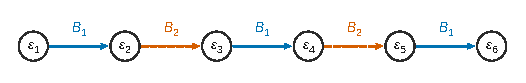
\includegraphics{figures/q20-decomposition-jn.pdf}
\caption*{Figure 2 --- J\_6 vue comme la chaîne ε\_1 → \ldots{} → ε\_6 : B\_1
(bleu, plein) prend les flèches issues d'un indice impair, B\_2 (orange,
tirets) celles d'un indice pair}
\end{figure}

\hypertarget{question-21}{%
\subsection{Question 21}\label{question-21}}

Posons
\equationajustee{\begin{aligned}B_1&=\sum_{\substack{j\le n-2\\ j\text{ impair}}}E_{j+1,j}+\sum_{\substack{i\le n-1\\ i\text{ pair}}}c_iE_{i,n},\\ B_2&=\sum_{\substack{j\le n-2\\ j\text{ pair}}}E_{j+1,j}+\sum_{\substack{i\le n-1\\ i\text{ impair}}}c_iE_{i,n}.\end{aligned}}

Clairement \(B_1+B_2=V+E_C\). Lisons \(B_1\) sur la base canonique \((\varepsilon_j)\) :

\begin{itemize}
\tightlist
\item
  pour \(j\le n-2\) impair, \(B_1\varepsilon_j=\varepsilon_{j+1}\), avec \(j+1\le n-1\) pair ;
\item
  pour \(j\le n-1\) pair, ou \(j=n-1\), \(B_1\varepsilon_j=0\) ;
\item
  \(B_1\varepsilon_n=\sum_{i\le n-1,\ i\text{ pair}}c_i\varepsilon_i\).
\end{itemize}

Ainsi \(B_1\) envoie chaque \(\varepsilon_j\) dans \(\operatorname{Vect}(\varepsilon_i:\ i\le n-1,\allowbreak \ i\text{ pair})\). Or \(B_1\) annule tous ces \(\varepsilon_i\). Donc \(B_1^2=0\).

Symétriquement, \(B_2\) envoie chaque \(\varepsilon_j\) dans \(\operatorname{Vect}(\varepsilon_i:\ i\le n-1,\allowbreak \ i\text{ impair})\).

Ce sous-espace est annulé par \(B_2\) : pour \(i\) impair, \(i\) n'est pas une colonne paire \(\le n-2\) et \(i\neq n\), donc \(B_2\varepsilon_i=0\).

Ainsi \(B_2^2=0\).
\equationajustee{\boxed{\begin{aligned}{}&V+E_C=B_1+B_2,\\ &B_1^2=B_2^2=0.\end{aligned}}}

\begin{figure}[H]
\centering
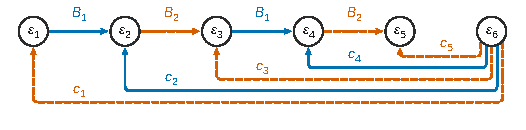
\includegraphics{figures/q21-decomposition-v-ec.pdf}
\caption*{Figure 3 --- V + E\_C pour n = 6 : la chaîne s'arrête en ε\_5, les
retours ε\_6 → ε\_i de poids c\_i vont dans B\_1 si i est pair, dans
B\_2 si i est impair}
\end{figure}

\hypertarget{question-22}{%
\subsection{Question 22}\label{question-22}}

\(v\) n'étant pas une homothétie, \(n\ge2\). Comme \(\chi_v\) est scindé sur \(\mathbb C\), on distingue deux cas.

\emph{Cas 1 : \(v\) a deux valeurs propres distinctes \(\lambda\neq\mu\)}, de vecteurs propres \(x\) et \(y\).

Ces vecteurs forment une famille libre, et \(P=\operatorname{Vect}(x,y)\) est un plan stable. Le vecteur \(z=x+y\neq0\) n'est pas propre.

En effet, \(v(z)=\nu z\) donnerait \(\lambda x+\mu y=\nu x+\nu y\), donc \(\lambda=\nu=\mu\) par liberté, ce qui est exclu.

\emph{Cas 2 : \(v\) a une seule valeur propre \(\lambda\).} Alors \(\chi_v=(X-\lambda)^n\). Soit \((h_1,\dots,h_n)\) une base de trigonalisation et \(H_k=\operatorname{Vect}(h_1,\dots,h_k)\).

La matrice de \(N=v-\lambda\,\mathrm{id}\) y est triangulaire supérieure stricte. Donc \(N(H_k)\subset H_{k-1}\), puis \(N^n=0\).

De plus \(N\neq0\) car \(v\) n'est pas une homothétie.

Soit \(y\) avec \(Ny\neq0\), et \(p\ge1\) le plus grand entier tel que \(N^py\neq0\) (on a \(p\le n-1\)).

Le vecteur \(x=N^{p-1}y\) vérifie \(Nx\neq0\) et \(N^2x=0\).

La famille \((x,Nx)\) est libre. Si \(\alpha x+\beta Nx=0\), appliquer \(N\) donne \(\alpha Nx=0\), donc \(\alpha=0\), puis \(\beta=0\).

Le plan \(P=\operatorname{Vect}(x,Nx)\) est stable, car
\equationajustee{\begin{aligned}v(x)&=\lambda x+Nx,\\ v(Nx)&=\lambda Nx.\end{aligned}}

Enfin \(x\) n'est pas propre : \(v(x)=\nu x\) donnerait \(Nx=(\nu-\lambda)x\), contraire à la liberté de \((x,Nx)\).

\textbf{Dans les deux cas, il existe un plan stable par \(v\) contenant un vecteur non nul qui n'est pas vecteur propre de \(v\).}

\hypertarget{question-23}{%
\subsection{Question 23}\label{question-23}}

Soit \(M\notin\operatorname{Vect}(I_n)\) et \(v\) l'endomorphisme canoniquement associé : \(v\) n'est pas une homothétie.

Par Q22, soit \(P\) un plan stable et \(f_1\in P\) non nul et non propre. Alors \(f_2=v(f_1)\in P\), et \((f_1,f_2)\) est libre, sinon \(f_1\) serait propre : c'est une base de \(P\).

On la complète en une base \(\mathcal F=(f_1,\dots,f_n)\). Comme \(v(P)\subset P\),
\equationajustee{\begin{aligned}\operatorname{Mat}_{\mathcal F}(v)&=\begin{pmatrix}B&D\\0&C'\end{pmatrix},\\ B&=\begin{pmatrix}0&b_{1,2}\\1&b_{2,2}\end{pmatrix}.\end{aligned}}
Puisque \(v(f_1)=f_2\), on a \(b_{2,1}=1\neq0\).

La matrice \(C'\in\mathcal M_{n-2}(\mathbb C)\) est trigonalisable : \(C'=QCQ^{-1}\) avec \(C\) triangulaire supérieure. Avec \(R=\begin{pmatrix}I_2&0\\0&Q\end{pmatrix}\),
\equationajustee{R^{-1}\begin{pmatrix}B&D\\0&C'\end{pmatrix}R=\begin{pmatrix}B&DQ\\0&C\end{pmatrix}.}

Par transitivité de la similitude, \(M\) est semblable à
\equationajustee{\boxed{\begin{pmatrix}B&(?)\\(0)&C\end{pmatrix},\ \text{avec}\ b_{2,1}\neq0\ \text{et}\ C\ \text{triangulaire \text{supérieure}.}}}
(Pour \(n=2\), le bloc \(C\) est vide.)

\hypertarget{question-24}{%
\subsection{Question 24}\label{question-24}}

Soit \(M\notin\operatorname{Vect}(I_n)\). Alors \(M^\top\notin\operatorname{Vect}(I_n)\).

Par Q23, il existe \(S\in GL_n(\mathbb C)\) telle que \(M^\top=SNS^{-1}\), avec \(N=\begin{pmatrix}B&X\\0&C\end{pmatrix}\), \(b_{2,1}\neq0\) et \(C\) triangulaire supérieure.

En transposant, \(M=(S^\top)^{-1}N^\top S^\top\) : \(M\) est semblable à
\equationajustee{N^\top=\begin{pmatrix}B^\top&0\\X^\top&C^\top\end{pmatrix}.}

Au-dessus de la diagonale, \(N^\top\) n'a qu'un seul coefficient éventuellement non nul : le coefficient \((1,2)\), égal à \(b_{2,1}\neq0\). En effet, le bloc en haut à droite est nul et \(C^\top\) est triangulaire inférieure.

Soit \(W=\sum_{i=1}^nE_{i,n+1-i}\), matrice de la permutation \(i\mapsto n+1-i\). On a \(W^2=I_n\) et
\equationajustee{(WN^\top W)_{i,j}=(N^\top)_{n+1-i,\,n+1-j}.}

Pour \(i>j\), on a \(n+1-i<n+1-j\). Ce coefficient est donc nul, sauf si \((n+1-i,n+1-j)=(1,2)\), c'est-à-dire \((i,j)=(n,n-1)\), où il vaut \(b_{2,1}\neq0\).

Donc \(A=WN^\top W\) est presque triangulaire supérieure, et
\equationajustee{\boxed{M\ \text{est semblable \text{à} la matrice presque triangulaire \text{supérieure}}\ A=WN^\top W.}}

\hypertarget{question-25}{%
\subsection{Question 25}\label{question-25}}

Soit \(u\in\mathcal L(E)\) de trace nulle, \(n=\dim E\).

\emph{Homothéties.} Si \(u=\lambda\,{\mathrm{id}}_E\), alors \(n\lambda=0\), donc \(u=0=0+0+0+0\in\Sigma_4\mathcal C(E)\). Cela règle en particulier le cas \(n=1\).

\emph{Cas général} (\(n\ge2\), \(u\) non homothétique). Soit \(M\) la matrice de \(u\) dans une base : \(M\notin\operatorname{Vect}(I_n)\) et \(\operatorname{tr}M=0\).

Par Q24, \(M=SAS^{-1}\) avec \(A\) presque triangulaire supérieure, et \(\operatorname{tr}A=\operatorname{tr}M=0\).

Par Q19, il existe \(C_0\) et \(Q\in GL_n(\mathbb C)\) tels que \(A+V+E_{C_0}=QJ_nQ^{-1}\).

Par Q20, \(J_n=B_1+B_2\), et par Q21, \(V+E_{C_0}=B_3+B_4\), avec \(B_k^2=0\) pour \(k=1,2,3,4\). Donc
\equationajustee{A=QB_1Q^{-1}+QB_2Q^{-1}+(-B_3)+(-B_4).}

C'est une somme de quatre matrices de carré nul, car \((QB_kQ^{-1})^2=QB_k^2Q^{-1}=0\) et \((-B_k)^2=B_k^2=0\). Puis
\equationajustee{M=SQB_1(SQ)^{-1}+SQB_2(SQ)^{-1}-SB_3S^{-1}-SB_4S^{-1},}
encore somme de quatre matrices de carré nul.

Par l'isomorphisme d'algèbres \(f\mapsto\operatorname{Mat}(f)\), on obtient \(u=u_1+u_2+u_3+u_4\) avec \(u_k\in\mathcal C(E)\) :
\equationajustee{\boxed{u\in\Sigma_4\mathcal C(E).}}

Avec Q8 et Q13, pour \(n\ge5\) :
\equationajustee{\begin{aligned}{}&\Sigma_3\mathcal C(E)\subsetneq\Sigma_4\mathcal C(E),\\ &\Sigma_4\mathcal C(E)=\Sigma_\infty\mathcal C(E)=\mathcal H(E),\end{aligned}}
et le nombre \(4\) est optimal.

\end{document}
